%%===========================================================%%
%%                                                           %%
%%                   SYSTEMATIC ERRORS                       %%
%%                                                           %%
%%===========================================================%%


\chapter{Systematic errors}\label{chap:systematicErrors}
\section{TPC track reconstruction efficiency}\label{sec:tpcSystematics}
\subsection{Embedding (pile-up) effect}\label{subsec:TpcEffSystPileUp}
One major difference between simulation and real data is the presence of pile-up
events. The average number of pile-up tracks in
a triggering event is proportional to the BBC coincidence rate. It is expected that
the difference between simulation and real data drops at lower BBC rates, and the
effects of pile-up tracks could be much reduced by fitting the tracking efficiency as a
function of BBC rate and using the extrapolated value at zero luminosity to compare
with simulation.\newline

%---------------------------
\begin{wrapfigure}{r}{0.45\textwidth}\vspace*{-9pt}
	\centering
	\includegraphics[width=0.45\textwidth, page=5]{graphics/systematicsEfficiency/bbc_and/Out.pdf}
	\caption[Number of events in embedded MC as a function of BBC\_AND rate.]
	{Number of events in embedded MC as a function of BBC\_AND rate. The black and red lines represent the events with \mbox{$<\text{BBC\_AND}>=700$~kHz} and \mbox{$<\text{BBC\_AND}>=1400$~kHz},  respectively.}
	\label{fig:events_bbc_and}%\vspace*{-29pt}
\end{wrapfigure}
%---------------------------
\noindent The embedded MC was divided into two samples due to mean BBC\_AND rate: \mbox{$<\text{BBC\_AND}>=700$~kHz} and \mbox{$<\text{BBC\_AND}>=1400$~kHz}. Next, the track reconstruction efficiency was calculated for those two samples and no-pile-up MC corresponding to them. The difference between TPC track reconstruction efficiences for pile-up and no-pile-up MCs was calculated as:
\begin{equation}
	\Delta\epsilon_{ TPC}^{1400/700\text{ kHz}} = \frac{N_{reco}^{no-pile-up}-N_{reco}^{pile-up}}{N_{gen}}\\
	\label{eq:tpcSyst}
\end{equation}
where:\\
$N_{gen}$-number of MC tracks,\\
$N_{reco}^{no-pile-up}$ - number of reconstructed tracks, matched with MC tracks in no-pile-up MC,\\
$N_{reco}^{pile-up}$ - number of reconstructed tracks, matched with MC tracks in pile-up MC.

The difference between high and low pile-up runs is given by:
\begin{equation}
\Delta\epsilon_{ TPC} =\Delta\epsilon_{ TPC}^{1400\text{ kHz}}-2\cdot\Delta\epsilon_{ TPC}^{700\text{ kHz}}
\label{eq:tpcSystDifference}
\end{equation}
Finally, above difference, shown in  \Cref{fig:systError1Dtpc,fig:systError2Dtpc} for $\pi^\pm$, varies between $2-3\%$ and was taken as systematic uncertainty related to TPC track reconstruction efficiency.
%\vspace{10em}
\begin{figure}[hb]
	\caption[$\pi^\pm$ TPC track reconstruction efficiency as a function of $p_T$ $\left(|\eta|<0.7, |V_z|<80\text{ cm}\right)$ for embedded MC samples with \mbox{$<\text{BBC\_AND}>=700$~kHz} and \mbox{$<\text{BBC\_AND}>=1400$~kHz}]{$\pi^\pm$ TPC track reconstruction efficiency as a function of $p_T$ $\left(|\eta|<0.7, |V_z|<80\text{ cm}\right)$ for embedded MC samples with \mbox{$<\text{BBC\_AND}>=700$~kHz} and \mbox{$<\text{BBC\_AND}>=1400$~kHz}. The efficiences from corresponding no-pile-up MC samples were also shown. Additionally, the differences  from Eq. \ref{eq:tpcSystDifference} were drawn in the bottom of each plot.}
	\label{fig:systError1Dtpc}
	\centering
	\parbox{0.495\textwidth}{
		\centering
		\includegraphics[width=\linewidth,page=1]{graphics/systematicsEfficiency/bbc_and/tpcEffi_d0_1_5_etapt_1.pdf}\\
	}~
	\parbox{0.495\textwidth}{
		\centering
		\includegraphics[width=\linewidth,page=2]{graphics/systematicsEfficiency/bbc_and/tpcEffi_d0_1_5_etapt_1.pdf}\\
	}%
\end{figure}
\begin{figure}[H]
	\caption[The difference $\Delta\epsilon_{ TPC} =\Delta\epsilon_{ TPC}^{1400\text{ kHz}}-2\cdot\Delta\epsilon_{ TPC}^{700\text{ kHz}}$ for $\pi^\pm$ as a function of $p_T$ and $\eta$ $\left(|V_z|<80\text{ cm}\right)$]{The difference $\Delta\epsilon_{ TPC} =\Delta\epsilon_{ TPC}^{1400\text{ kHz}}-2\cdot\Delta\epsilon_{ TPC}^{700\text{ kHz}}$ for $\pi^\pm$ as a function of $p_T$ and $\eta$ $\left(|V_z|<80\text{ cm}\right)$. }
	\label{fig:systError2Dtpc}
	\centering
	\parbox{0.495\textwidth}{
		\centering
		\includegraphics[width=\linewidth,page=1]{graphics/systematicsEfficiency/bbc_and/tpcEffi_d0_1_5_etapt_12D.pdf}\\
	}~
	\parbox{0.495\textwidth}{
		\centering
		\includegraphics[width=\linewidth,page=2]{graphics/systematicsEfficiency/bbc_and/tpcEffi_d0_1_5_etapt_12D.pdf}\\
	}%
\end{figure}

\subsection{Dead material effect on TPC track reconstruction efficiency}\label{sec:deadMaterialSystematics}
The amount of dead material in front of TPC differs up to $20\%$ between data and simulation (see Sec.~\ref{chap:deadMaterial}). First, the~amount of lost particles, $\delta\epsilon_{ TPC}$, due to the interaction with dead material in front of TPC was estimated using  no-pile-up  MC samples. The results for $\pi^-$ in CD are shown in Fig. \ref{fig:dead_materialCD3D}. Then the symmetric systematic uncertainty to the TPC track reconstruction efficiency due to dead material was introduced as $\pm 0.2 \cdot\delta\epsilon_{ TPC}$.
In Fig. \ref{fig:dead_materialCD1D}  the systematic uncertainty is shown for each particle species in CD as a function of $p_T$ $\left(|\eta|<0.7, |V_{z}|<80 \text{ cm}\right)$. 
The results for other particles and SD are shown in Figs. in Appendix \ref{appendix:deadMaterial}.
\begin{figure}[hb]
\caption[The amount of lost $\pi^-$ due to the interaction with dead material in front of TPC as a function of $p_T$, $\eta$ and $z$-vertex in CD]{The amount of lost $\pi^-$ due to the interaction with dead material in front of TPC. Each plot represents the fraction of lost $\pi^-$, $\delta\epsilon_{ TPC}$ ($z$-axis), as a function of true particle pseudorapidity $\eta$ ($y$-axis) and transverse momentum $p_{T}$ ($x$-axis) in single $z$-vertex bin.}\label{fig:dead_materialCD3D}
\centering
\parbox{0.495\textwidth}{
  \centering
  \includegraphics[width=\linewidth,page=1]{graphics/systematicsEfficiency/deadMaterial/secondaries_Unbinned_CD_.pdf}\\
  \includegraphics[width=\linewidth,page=3]{graphics/systematicsEfficiency/deadMaterial/secondaries_Unbinned_CD_.pdf}\\
  \includegraphics[width=\linewidth,page=5]{graphics/systematicsEfficiency/deadMaterial/secondaries_Unbinned_CD_.pdf}\\
  \includegraphics[width=\linewidth,page=7]{graphics/systematicsEfficiency/deadMaterial/secondaries_Unbinned_CD_.pdf}\\
}~
\parbox{0.495\textwidth}{
  \centering
  \includegraphics[width=\linewidth,page=2]{graphics/systematicsEfficiency/deadMaterial/secondaries_Unbinned_CD_.pdf}\\
  \includegraphics[width=\linewidth,page=4]{graphics/systematicsEfficiency/deadMaterial/secondaries_Unbinned_CD_.pdf}\\
  \includegraphics[width=\linewidth,page=6]{graphics/systematicsEfficiency/deadMaterial/secondaries_Unbinned_CD_.pdf}\\
  \includegraphics[width=\linewidth,page=8]{graphics/systematicsEfficiency/deadMaterial/secondaries_Unbinned_CD_.pdf}
}%
\end{figure}
\begin{figure}[hb]\ContinuedFloat
% ~\\[32pt]
\centering
\parbox{0.495\textwidth}{
  \centering
  \includegraphics[width=\linewidth,page=9]{graphics/systematicsEfficiency/deadMaterial/secondaries_Unbinned_CD_.pdf}\\
  \includegraphics[width=\linewidth,page=11]{graphics/systematicsEfficiency/deadMaterial/secondaries_Unbinned_CD_.pdf}\\
  \includegraphics[width=\linewidth,page=13]{graphics/systematicsEfficiency/deadMaterial/secondaries_Unbinned_CD_.pdf}\\
  \includegraphics[width=\linewidth,page=15]{graphics/systematicsEfficiency/deadMaterial/secondaries_Unbinned_CD_.pdf}\\
}~
\parbox{0.495\textwidth}{
  \centering
  \includegraphics[width=\linewidth,page=10]{graphics/systematicsEfficiency/deadMaterial/secondaries_Unbinned_CD_.pdf}\\
  \includegraphics[width=\linewidth,page=12]{graphics/systematicsEfficiency/deadMaterial/secondaries_Unbinned_CD_.pdf}\\
  \includegraphics[width=\linewidth,page=14]{graphics/systematicsEfficiency/deadMaterial/secondaries_Unbinned_CD_.pdf}\\
  \includegraphics[width=\linewidth,page=16]{graphics/systematicsEfficiency/deadMaterial/secondaries_Unbinned_CD_.pdf}
}%
\end{figure}
\begin{figure}[hb]
\caption[The systematic uncertainty to the TPC track reconstruction efficiency due to  amount of dead material in front of TPC using MC samples for CD]{The systematic uncertainty to the TPC track reconstruction efficiency due to  amount of dead material in front of TPC using MC samples for CD. Each plot represents the systematic uncertainty as a~function of true particle $p_T$ $\left(|\eta|<0.7, |V_{z}|<80 \text{ cm}\right)$ for given particle species: $\pi^-$,$\pi^+$, $K^-$, $K^+$, $\bar{p}$ and $p$. It was also calculated for negative and positive particles without identification. }\label{fig:dead_materialCD1D}
\centering
\parbox{0.495\textwidth}{
  \centering
  \includegraphics[width=\linewidth,page=1]{graphics/systematicsEfficiency/deadMaterial/secondaries_Unbinned_CD_1D.pdf}\\
  \includegraphics[width=\linewidth,page=2]{graphics/systematicsEfficiency/deadMaterial/secondaries_Unbinned_CD_1D.pdf}\\
  \includegraphics[width=\linewidth,page=3]{graphics/systematicsEfficiency/deadMaterial/secondaries_Unbinned_CD_1D.pdf}\\
  \includegraphics[width=\linewidth,page=1]{graphics/systematicsEfficiency/deadMaterial/secondaries_Unbinned_Charged_CD1D.pdf}\\
}~
\parbox{0.495\textwidth}{
  \centering
  \includegraphics[width=\linewidth,page=4]{graphics/systematicsEfficiency/deadMaterial/secondaries_Unbinned_CD_1D.pdf}\\
  \includegraphics[width=\linewidth,page=5]{graphics/systematicsEfficiency/deadMaterial/secondaries_Unbinned_CD_1D.pdf}\\
  \includegraphics[width=\linewidth,page=6]{graphics/systematicsEfficiency/deadMaterial/secondaries_Unbinned_CD_1D.pdf}\\
  \includegraphics[width=\linewidth,page=2]{graphics/systematicsEfficiency/deadMaterial/secondaries_Unbinned_Charged_CD1D.pdf}
}%
\end{figure}



\section{TOF matching efficiency}\label{sec:tofSystematics}
\subsection{Embedding (pile-up) effect}
The approach to calculate the systematic uncertainty on TOF matching efficiency related to pile-up was quite similar to the one used for TPC track reconstruction efficiency (Sec.~\ref{subsec:TpcEffSystPileUp}). However, the TOF matching efficiency is conditional and depends on TPC track reconstruction efficiency. Since that, the difference between high and low pile-up runs is given by:
\begin{equation}
\Delta\epsilon_{ TOF}^{1400/700\text{ kHz}}=\frac{N_{TPC-TOF}^{no-pile-up}}{N_{TPC}^{no-pile-up}}-\frac{N_{TPC-TOF}^{pile-up}}{N_{TPC}^{pile-up}}
\label{eq:tofSyst}
\end{equation}
where:\\
$N_{TPC-TOF}^{pile-up}$ - number of reconstructed tracks, matched with MC tracks and TOF hit in pile-up MC,\\
$N_{TPC-TOF}^{no-pile-up}$ - number of reconstructed tracks, matched with MC tracks and TOF hit in no-pile-up MC,\\
$N_{TPC}^{pile-up}$ - number of reconstructed tracks, matched with MC tracks in pile-up MC,\\
$N_{TPC}^{no-pile-up}$ - number of reconstructed tracks, matched with MC tracks in no-pile-up MC.

\noindent Next the difference between high and low pile-up events was calculated withe the formula similar to the one given by Eq. \ref{eq:tpcSystDifference} and is shown in \Cref{fig:systError1Dtof,fig:systError2Dtof}. The origin of  $N_{TPC-TOF}$ increase is not known (it may be due to lack of pile-up in TPC or TOF). Since that, it is impossible to correctly calculate the statistical error for $\Delta\epsilon_{ TOF}$. Nevertheless, $\Delta\epsilon_{ TOF}$ is  smaller than $0.5\%$ and can be neglected in comparison with other systematic uncertainties.
\begin{figure}[hb]
	\caption[$\pi^\pm$ TOF matching efficiency as a function of $p_T$ $\left(|\eta|<0.7, |V_z|<80\text{ cm}\right)$ for embedded MC samples with \mbox{$<\text{BBC\_AND}>=700$~kHz} and \mbox{$<\text{BBC\_AND}>=1400$~kHz}]{$\pi^\pm$ TOF matching efficiency as a function of $p_T$ $\left(|\eta|<0.7, |V_z|<80\text{ cm}\right)$ for embedded MC samples with \mbox{$<\text{BBC\_AND}>=700$~kHz} and \mbox{$<\text{BBC\_AND}>=1400$~kHz}. The efficiences from corresponding no-pile-up MC samples were also shown. Additionally, the differences  from Eq. \ref{eq:tpcSystDifference} were drawn in the bottom of each plot.}
	\label{fig:systError1Dtof}
	\centering
	\parbox{0.495\textwidth}{
		\centering
		\includegraphics[width=\linewidth,page=1]{graphics/systematicsEfficiency/bbc_and/tofEffi_d0_1_5_etapt_1.pdf}\\
	}~
	\parbox{0.495\textwidth}{
		\centering
		\includegraphics[width=\linewidth,page=2]{graphics/systematicsEfficiency/bbc_and/tofEffi_d0_1_5_etapt_1.pdf}\\
	}%
\end{figure}
\begin{figure}[H]
	\caption[The difference $\Delta\epsilon_{ TOF} =\Delta\epsilon_{ TOF}^{1400\text{ kHz}}-2\cdot\Delta\epsilon_{ TOF}^{700\text{ kHz}}$ for $\pi^\pm$ as a function of $p_T$ and $\eta$ $\left(|V_z|<80\text{ cm}\right)$]{The difference $\Delta\epsilon_{ TOF} =\Delta\epsilon_{ TOF}^{1400\text{ kHz}}-2\cdot\Delta\epsilon_{ TOF}^{700\text{ kHz}}$ for $\pi^\pm$ as a function of $p_T$ and $\eta$ $\left(|V_z|<80\text{ cm}\right)$. }
	\label{fig:systError2Dtof}
	\centering
	\parbox{0.495\textwidth}{
		\centering
		\includegraphics[width=\linewidth,page=1]{graphics/systematicsEfficiency/bbc_and/tofEffi_d0_1_5_etapt_12D.pdf}\\
	}~
	\parbox{0.495\textwidth}{
		\centering
		\includegraphics[width=\linewidth,page=2]{graphics/systematicsEfficiency/bbc_and/tofEffi_d0_1_5_etapt_12D.pdf}\\
	}%
\end{figure}



\subsection{Simulation accuracy (absolute error on TOF efficiency)}

The efficiency of TOF hit reconstruction and matching with the TPC tracks that was used in our analyses was taken directly from the STAR simulation. This makes the inaccuracies in the description of real detector geometry and its response propagating to physics results and introducing a bias. We decided to estimate the systematic uncertainty connected with the accuracy of description of the TOF system in (data-embedded) STAR simulation by extracting the TOF efficiency in the very same way from the data and embedded MC and comparing the results.

Unfortunately, in 2015 there were no low-luminosity (heavy-ion) runs that would imply lack of off-time pile-up tracks in TPC and thus would allow calculating the TOF efficiency in straightforward way, namely by dividing number of selected TPC tracks that were matched with TOF hits by number of all selected TPC tracks (matched or unmatched). For this reason a variation of the ``tag and probe'' method was developed and used.

%---------------------------
\begin{figure}[b!]%\vspace{-2pt}%
\centering%
\begin{minipage}{.4725\textwidth}%
  \centering%\vspace{11pt}
  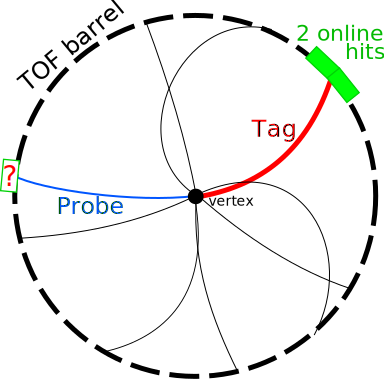
\includegraphics[width=0.98\linewidth]{graphics/systematicsEfficiency/TOF_tagAndProbe/sketch.pdf}%\vspace{-5pt}%
  \caption[Sketch of the tag\&probe method.]%
  {Sketch of the cross section of the central detector and CEP event with off-time pile-up tracks with drafted tag\&probe method used to determine the TOF hit reconstruction and matching efficiency.\newline }\label{fig:tagAndProbeSketch}
\end{minipage}%
\quad\quad%
\begin{minipage}{.4725\textwidth}%
  \centering%
  \includegraphics[width=\linewidth]{graphics/systematicsEfficiency/TOF_tagAndProbe/TofMultOfflineVsOnline.pdf}%\vspace*{-5pt}
  \caption[Comparison of original and reconstructed TOF multiplicity at the trigger level.]
   {Comparison of original online TOF multiplicity at L0 (horizontal axis) and TOF multiplicity reconstructed from the offline hits (vertical axis) for preselected RP\_CPT triggers (at least 1 primary vertex with TOF-matched TPC tracks).}
   \label{fig:tofOnlineMultRecoVsL0}%\vspace*{-29pt}
\end{minipage}%
\end{figure}%
%---------------------------

The mentioned tag\&probe method made use of the CEP of $\pi^{+}\pi^{-}$ events. In short, events with forward proton track on each side of STAR and with a TOF-matched primary TPC track (tag) were selected. Among the remaining primary TPC tracks in the same vertex the opposite-sign TPC track (probe) was chosen as the one which provides the minimum total transverse momentum of all four tracks. The probe was checked whether it has been matched with the TOF hit or not. The ratio of the matched TPC tracks to all (matched or unmatched) TPC tracks defined the TOF efficiency. The method is illustrated in the sketch in Fig.~\ref{fig:tagAndProbeSketch}. The detailed description of the procedure of the TOF efficiency extraction is provided below:

\begin{enumerate}
 \item Data from two triggers were used (independently): RP\_CPT and RP\_CPT2 (trigger details in Tab.~2.1 of Ref.~\cite{AnalysisNoteRafal}). Embedded $\pi^{+}\pi^{-}$ GenEx MC sample was subjected to the same trigger conditions (depending on the data to be compared with). Since there is no simulation of the TOF trigger we used in MC analysis L0 TOF multiplicity reconstructed from the offline hits according to TOF trigger system description (see Ref.~\cite{tofL0MultExplanation}). In Fig.~\ref{fig:tofOnlineMultRecoVsL0} we show performance of implemented method of L0 TOF multiplicity reconstruction. One can find satisfactory correlation of the true multiplicity and the reconstructed one.
 \item Events were selected with the following set of cuts from nominal CEP analysis (Ref.~\cite{AnalysisNoteRafal}): \textbf{C1}, \textbf{C2} (TPC vertex), \textbf{C4} (RP tracks), \textbf{C5} (TPC-RP vertex matching), \textbf{C6} (veto signal in large BBC), providing significant reduction of background events.
 \item 
\end{enumerate}

\begin{equation}\label{eq:tofEffFunc}
 \varepsilon^{TOF}(p_{T}) = A\cdot \exp\Big\{-\left(B/p_{T}\right)^{C}\Big\}
\end{equation}




%---------------------------
\begin{figure}[h!]
\centering
\parbox{0.4725\textwidth}{
  \centering
  \begin{subfigure}[b]{\linewidth}{
                \subcaptionbox{\label{fig:tofEffSystVsPt_CPT}}{\includegraphics[width=\linewidth]{graphics/systematicsEfficiency/TOF_tagAndProbe/CPT/TofEffVsPt.pdf}\vspace{-5pt}}}
  \end{subfigure}\\[3pt]
  \begin{subfigure}[b]{\linewidth}\addtocounter{subfigure}{1}{
                \subcaptionbox{\label{fig:tofEffSystVsEta_CPT}}{\includegraphics[width=\linewidth]{graphics/systematicsEfficiency/TOF_tagAndProbe/CPT/TofEffVsEta.pdf}\vspace{-5pt}}}
  \end{subfigure}
}
\quad
\parbox{0.4725\textwidth}{
  \centering
  \begin{subfigure}[b]{\linewidth}\addtocounter{subfigure}{-2}{
                \subcaptionbox{\label{fig:tofEffSystVsPt_CPT2}}{\includegraphics[width=\linewidth]{graphics/systematicsEfficiency/TOF_tagAndProbe/CPT2/TofEffVsPt.pdf}\vspace{-5pt}}}
  \end{subfigure}\\[3pt]
  \begin{subfigure}[b]{\linewidth}\addtocounter{subfigure}{1}{
                \subcaptionbox{\label{fig:tofEffSystVsEta_CPT2}}{\includegraphics[width=\linewidth]{graphics/systematicsEfficiency/TOF_tagAndProbe/CPT2/TofEffVsEta.pdf}\vspace{-5pt}}}
  \end{subfigure}
}%\vspace{-5pt}%
\caption[Tag\&Probe TOF efficiency from CEP data compared with the result from embedded CEP MC.]%
    {Tag\&Probe TOF efficiency from CEP data (black points) compared with the result from embedded CEP MC (red points) as a function of TPC track $p_{T}$ (top row) and $\eta$ (bottom row). The left and right hand side column represents results obtained from RP\_CPT and RP\_CPT2 triggers, respectively. Green points represent the TOF efficiency calculated in the standard way from embedded CEP MC sample. Blue lines denote the TOF efficiency calculated in the standard way solely from the selected probe tracks that were matched to primary pions at the true level. Difference between red points and blue lines show the potential bias of tag and probe method. Dashed lines are fits of function given by Eq.~\eqref{eq:tofEffFunc} to points of corresponding color. Dashed vertical lines with arrows indicate region of $p_{T}$ and $\eta$ accepted in analyses.}\label{fig:tofEffSyst}%
\end{figure}
%---------------------------

% %---------------------------
% \begin{figure}[h!]
% \centering
% \parbox{0.4725\textwidth}{
%   \centering
%   \begin{subfigure}[b]{\linewidth}
%                 \subcaptionbox{\label{fig:tofEffSystVsPt}}{\includegraphics[width=\linewidth]{graphics/systematicsEfficiency/TOF_tagAndProbe/TofEffVsPt.pdf}}\vspace{-5pt}
%   \end{subfigure}
% }%
% \quad\quad%
% \parbox{0.4725\textwidth}{
%   \centering
%   \begin{subfigure}[b]{\linewidth}
%                 \subcaptionbox{\label{fig:tofEffSystVsEta}}{\includegraphics[width=\linewidth]{graphics/systematicsEfficiency/TOF_tagAndProbe/TofEffVsEta.pdf}}\vspace{-5pt}
%   \end{subfigure}
% }%
% \caption[Tag\&Probe TOF efficiency from CEP data compared with the result from embedded CEP MC.]%
%     {Tag\&Probe TOF efficiency from CEP data (black points) compared with the result from embedded CEP MC (red points) as a function of TPC track $p_{T}$ (\ref{fig:tofEffSystVsPt}) and $\eta$ (\ref{fig:tofEffSystVsEta}). Green points represent the TOF efficiency calculated in the standard way from embedded CEP MC sample. Blue lines denote the TOF efficiency calculated in the standard way solely from the selected probe tracks that were matched to primary pions at the true level. Difference between red points and blue lines show the potential bias of tag and probe method.}\label{fig:tofEffSyst}%
% \end{figure}
% %---------------------------



%---------------------------
\begin{figure}[h!]
\centering
\parbox{0.4725\textwidth}{
  \centering
  \begin{subfigure}[b]{\linewidth}{
                \subcaptionbox{\label{fig:tofEffSystVsPt_negativeEta_CPT}}{\includegraphics[width=\linewidth]{graphics/systematicsEfficiency/TOF_tagAndProbe/CPT/TofEffVsPt_negativeEta.pdf}\vspace{-5pt}}}
  \end{subfigure}\\[3pt]
  \begin{subfigure}[b]{\linewidth}\addtocounter{subfigure}{1}{
                \subcaptionbox{\label{fig:tofEffSystVsPt_positiveEta_CPT}}{\includegraphics[width=\linewidth]{graphics/systematicsEfficiency/TOF_tagAndProbe/CPT/TofEffVsPt_positiveEta.pdf}\vspace{-5pt}}}
  \end{subfigure}
}
\quad
\parbox{0.4725\textwidth}{
  \centering
  \begin{subfigure}[b]{\linewidth}\addtocounter{subfigure}{-2}{
                \subcaptionbox{\label{fig:tofEffSystVsPt_negativeEta_CPT2}}{\includegraphics[width=\linewidth]{graphics/systematicsEfficiency/TOF_tagAndProbe/CPT2/TofEffVsPt_negativeEta.pdf}\vspace{-5pt}}}
  \end{subfigure}\\[3pt]
  \begin{subfigure}[b]{\linewidth}\addtocounter{subfigure}{1}{
                \subcaptionbox{\label{fig:tofEffSystVsPt_positiveEta_CPT2}}{\includegraphics[width=\linewidth]{graphics/systematicsEfficiency/TOF_tagAndProbe/CPT2/TofEffVsPt_positiveEta.pdf}\vspace{-5pt}}}
  \end{subfigure}
}%\vspace{-5pt}%
\caption[Tag\&Probe TOF efficiency from CEP data compared with the result from embedded CEP MC (divided w.r.t. $\eta$ of the probe).]%
    {Tag\&Probe TOF efficiency from CEP data (black points) compared with the result from embedded CEP MC (red points) as a function of TPC track $p_{T}$ for negative (top row) and positive (bottom row) $\eta$ of the probe. The left and right hand side column represents results obtained from RP\_CPT and RP\_CPT2 triggers, respectively. Blue lines denote the TOF efficiency calculated in the standard way solely from the selected probe tracks that were matched to primary pions at the true level. Difference between red points and blue lines show the potential bias of tag and probe method. Dashed lines are fits of function given by Eq.~\eqref{eq:tofEffFunc} to points of corresponding color. Dashed vertical lines with arrows indicate region of $p_{T}$ and $\eta$ accepted in analyses.}\label{fig:tofEffSyst_etaBins}%
\end{figure}
%---------------------------
% %---------------------------
% \begin{figure}[h!]
% \centering
% \parbox{0.4725\textwidth}{
%   \centering
%   \begin{subfigure}[b]{\linewidth}
%                 \subcaptionbox{\label{fig:tofEffSystVsPt_negativeEta}}{\includegraphics[width=\linewidth]{graphics/systematicsEfficiency/TOF_tagAndProbe/TofEffVsPt_negativeEta.pdf}}\vspace{-5pt}
%   \end{subfigure}
% }%
% \quad\quad%
% \parbox{0.4725\textwidth}{
%   \centering
%   \begin{subfigure}[b]{\linewidth}
%                 \subcaptionbox{\label{fig:tofEffSystVsPt_positiveEta}}{\includegraphics[width=\linewidth]{graphics/systematicsEfficiency/TOF_tagAndProbe/TofEffVsPt_positiveEta.pdf}}\vspace{-5pt}
%   \end{subfigure}
% }%
% \caption[ .]%
%     { .}\label{fig:tofEffSyst_etaBins}%
% \end{figure}
% %---------------------------